\documentclass[11pt, a4paper]{article} % Font size

\usepackage[utf8]{inputenc}
\usepackage[T1]{fontenc}
\usepackage[spanish,es-nolayout,es-nodecimaldot,es-tabla]{babel}
\usepackage{amsmath}
\usepackage{amsfonts}
\usepackage{amssymb,amsthm}
\usepackage{enumerate}
\usepackage{enumitem}
\usepackage{parskip}
\usepackage{nicefrac}
\usepackage[left=2cm,right=2cm,top=2.5cm,bottom=2cm]{geometry}
\usepackage{graphicx}
\linespread{1.25}

%%%

\begin{document}

La solución de la ecuación diferencial 

\begin{align}
	&y'(x)+2y(x)	=
	\left\{ \begin{aligned}
	1 \quad &si \quad x \in [0,3],
	\\ \nonumber
	0 \quad	&si \quad x > 3;
	\end{aligned}
	\right.
	\\\nonumber
	&\text{sujeta a}
	\\	\nonumber	
\end{align}
\vspace{-45pt}
					\[
					\hspace{-45pt}y(0)=0
					\]

está dada por la función a trozos

\[
	y(x)
	=
	\left\{ \begin{aligned}
	&\dfrac{1}{2}(e^{-2x} -1) \quad &si \quad x \leq 3,
	\\
	 &\dfrac{1}{2}(e^{-2x} -e^{6-2x}) \quad &si \quad x > 3;
	\end{aligned}
	\right.
\]

\begin{figure}[h]
\centering
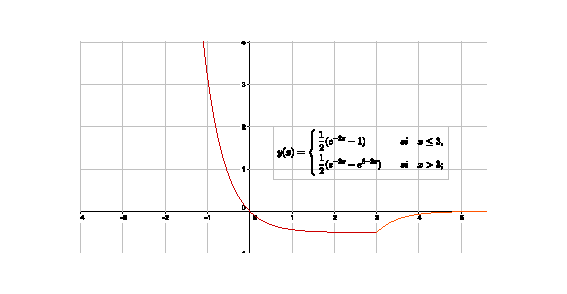
\includegraphics[scale=2]{grafico.pdf}
\end{figure}

\end{document}